%!TEX root = Funktionalanalysis - Vorlesung.tex

\chapter{Lineare Operatoren auf Banachräumen}
\section{Einführung}
\subsection{Räume}

Sei $X$ ein Vektorraum, $dim X < \infty $ und sei $x = (x_{1},\dotsc,x_{n})^{T} \in \MdR^{n}$
\begin{align*}
	& \|x\|_{2} := \left(\sum_{k = 1}^{n} \|x_{i}^{2}\| \right)^{\frac{1}{2}}\\
	& \|x\|_{\infty} := \smash{\displaystyle\max_{i = 1}^{n}}  \|x_{i}\|		
\end{align*}

Diese Normen sind äquivalent, denn:
$\| x \|_{\infty} \leq \| x \|_{2} \leq n^{\frac{1}{2}} \| x \|_{\infty}$ \newline

\begin{satz*}[Bolzano-Weierstraß] \label{s:1-bolzanoweierstrass}
$A \subset \MdR$ beschränkt. Dann hat jede Folge $(x_{n})_{n \in \MdN} \subset A$ eine konvergente Teilfolge.
\end{satz*}

\begin{beispiel}
$X = C[0, 1] = \{ f : [0, 1] \rightarrow \MdR: \text{ stetig auf } [0, 1] \}$
\begin{align*}
\| f \|_{2} & := \left( \int_{0}^{1} \| f(t) \|^{2} dt \right)^{\frac{1}{2}} \\
\| f \|_{\infty} & :=  \smash{\displaystyle\max_{t \in [0, 1]}}  \| f(t) \|
\end{align*}
\newline
Dabei gilt $\| f \|_{\infty} \leq \| f \|_{2}$ , aber mit folgender Funktion folgt zum Beispiel:$\hspace{0.25cm} f_n(t) = $ \\
	\begin{figure}[H]
		\centering
		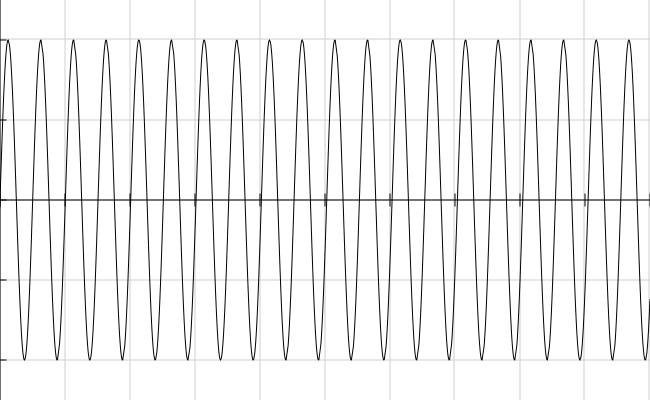
\includegraphics[width=160pt]{images/1.1.1-example1.png}
	\end{figure} \[ \| f_n \|_{\infty} = 1, \hspace{0.5cm} \| f_n \|_{2} \xrightarrow[n \rightarrow \infty]{} 0  
\hspace{0.5cm} \| f_{n} - f_{m} \| = 1 \text{ für } n \neq m \]
$ \Rightarrow $ \hyperref[s:1-bolzanoweierstrass]{Satz von Bolzano-Weierstraß} gilt im $\infty$-dimensionalen i.A. nicht!
\end{beispiel}

\subsection{Operatoren}

Sei $N = dim X, M = dim Y$ und seien $(e_n)$ bzw. $(f_n)$ Basen von $X$ bzw. $Y$. 	\\
Sei $T : X \rightarrow Y$ gegeben durch: \\
\[ \begin{xy} \xymatrix{
	X \ar[r]^T	\ar[d]_{ \alpha_{n} \rightarrow \sum \alpha_{n} e_{n} }  &   Y \ar[d]^{ \beta_{n} \rightarrow \sum \beta_{n} f_{n} }  \\
      	\MdR^{N} 	\ar[r]^A    				&   \MdR^{n}  				
} \end{xy} \]
wobei $x = \sum \alpha_{n} e_{n},\hspace{0.2cm} Tx = \sum \beta_n f_n, \hspace{0.2cm} \beta_m = \sum_{n = 1}^{N} a_{mn} \alpha_{n}. $ \\ \\
Daraus folgt:
\begin{itemize}
	\item $T$ ist stetig
	\item X = Y \gdw T injektiv \gdw T surjektiv (Dimensionsformel) \\
	(Die Gleichung $Tx = y$ ist eindeutig lösbar $\gdw$ Gleichung hat für alle $y \in Y$ eine Lösung.)
	\item Falls A selbstadjungiert ist, d.h. $A = A^{*}$, gibt es eine Basis aus Eigenvektoren $(e_{n})$ von $A$, d.h. $ T( \sum_{n=1}^{N} \alpha_{n} e_{n} ) = \sum{n=1}^{N} \lambda_{n} \alpha_{n} e_{n}$, wobei $\lambda_{n}$ Eigenwerte sind $A =
			\begin{pmatrix}
				\diagentry{\lambda_{1}}\\
				&\diagentry{\xddots}\\
				&&\diagentry{\lambda_{n}}\\
			\end{pmatrix} $
\end{itemize}

\begin{beispiel}
$X = C^{1}[0, 1] = \{ f : [0, 1] \rightarrow \MdR: \text{ stetig auf } [0, 1] \}$ \\
$T f = f', T : X \rightarrow Y \text{ stetig.} $ (Aber: $T: C[0, 1] \rightarrow C[0, 1]$, hier ist $T$ nicht definiert.) \\

$T$ ist nicht stetig bzgl. $\| \cdot \|_{\infty}$-Norm, da:
\[ f_{n}(t) = \frac{1}{\sqrt{n}}e^{int}, \hspace{0.5cm}  \text{dann: } \|f_{n}\| \rightarrow 0 \text{ für } t \rightarrow \infty \]	
\[ T f_{n}(t) = i \sqrt{n} e^{int}, \hspace{0.5cm} \text{mit: } \| T f_{n} \|_{\infty} \rightarrow \infty, \text{ für } n \rightarrow \infty \]
\end{beispiel}

\begin{beispiel}
$X = L_{2} = \{ (a_{n}): \left( \sum_{n \geq 1}^{\infty} \| a_{n} \| \right)^{\frac{1}{2}} < \infty \}$	\\
$T ( a_{1}, a_{2}, a_{3}, ...) = ( 0, a_{1}, a_{2}, a_{3}, ...)$ \\

$T$ ist injektiv, aber nicht surjektiv
\end{beispiel}

\subsection{Anwendungen}

\begin{enumerate}
	\item Fredholm'sche Integralglechungen \\
	$X = C[0, 1], \hspace{0.25cm} k: [0, 1] \times [0, 1] \rightarrow \MdR$ stetig \\
	\[ Tf(t) = \int_{0}^{1} k(t, s) f(s) ds \]
	Analogie zum endlich dim. ('Verallg. der Matrixmultiplikation'):  $ T(f_{j})(i) = \sum_{j = 1}^{n} a_{ij}f_{j}$ \\ \\
 	$T$ ist in diesem Fall linear und stetig und es gilt die Fredholm'sche Alternative:
	\[ \lambda \in R \verb|\| \{0\}: (\lambda Id - T)(f) = y, \hspace{0.25cm} f,g \in C[0, 1] \]
	Dann existiert eine Lösung genau dann wenn diese eindeutig ist. \\
	\item Dirichletproblem \\
	$\Omega \subset \MdR^n$ Gebiet, offen, beschränkt, glatter Rand. Sei $g: \partial \Omega \rightarrow \MdR$ stetig \\ 
	Gesucht ist ein $f \in C(\bar \Omega) \bigcap  C^(\Omega)$, so dass $\nabla f = \sum_{i = 1}^{n} \frac{\partial^{2} f}{\partial x_{i}^2} = 0$ in $\Omega$ und $f_{\big| \partial \Omega}= g$ \\ \\
	Beispiel: Durch Wärmeverteilung auf dem Rand auf WV im Inneren schließen. \\ \\
	Lösung: Dirichletintegral $J(u) = \int_{\Omega} (\nabla u )^{2} dx$, wobei $ u \in M = \{ v \in C^{1}(\bar \Omega) | \hspace{0.25cm} v_{\big| \partial \Omega} = g \}$ \\
	Sei $v_{0}$ das absolute Minimum von $J$, d.h. $J(v_{0}) = \inf \{ J(w): w \in M \}$ \\
	$v \in C^{1}(\bar \Omega)$ mit $v = 0$ in einer Umgebung von $\partial U$. $\epsilon \rightarrow J(u_{0} + \epsilon v)$
	\[ \frac{d}{d\epsilon} J(u_{0} + \epsilon v) = \int_{\Omega} \frac{d}{d\epsilon} (\nabla u_{0} + \epsilon \nabla v)^{2} dx = 2 \int_{\Omega} (\nabla u_{0} + \epsilon \nabla v)(\nabla v) dx_{\big| \epsilon = 0} = 2 \int_\Omega (\nabla u_{0}) (\nabla v) dx \]
	Mit $0 \geq J(u_{0} + \epsilon v)- J(u_{0}) \geq 0: \hspace{0.25cm} \int (\nabla u_{0})(\nabla v) dx \overset{\text{P.I.}}{{=}} - \int (\nabla u_{0})v dx = 0$ \\
	\[ \Rightarrow \nabla u_{0} = 0 \text{, außerdem } u_{0 \hspace{0.1cm} \big| \partial \Omega} = g \text{ (s.o.)} \]
	Im allgemeinen exisitert da absolute Minimum $u_{0} \in J$ aber nicht. \\
	Ausweg: $X = \{ f \in L^{2}(\Omega), f' \in L^{2}(\Omega) \} \supset \{f \in C(\bar \Omega), f' \in C(\bar \Omega) \} $	\\
	In diesem Raum $X$ (Sobolevräume) gibt es ein Minimum $u_{0}$ von $J$. \\
	\item Sturm-Liouville Problem \\
	$X = C^{2}([0, 1]), Tu = (pu')' + qu$, mit $q \in C[0, 1], p \in C^{1}[0, 1]$ \\ 
	Problem: bei gegebenen $f \in C[0, 1]$ find $u \in X$ mit $Tu = f, v(0) = 0, v'(1) = 0$ \\ \\
	$Y = \{ f \in L^{2}[0, 1], f' \in L^{2}[0, 1] \}$ Hilbertraum. \\
	Orthonormalbais $(e_{n})$ von $Y$ wäre: $\| e_{n} \|_{2} = 1, \int e_{n}(x) e_{m}(x) dx = 0$ für $m \neq m$ \\
	$f \in Y: f = \sum_{n = 1}^{\infty} \alpha_{n} e_{n}$ mit $\| f \|^2 = \sum | \alpha_{n} |^2$ \\
	Die $(e_{n})$ sind außerdem Eigenvektoren des Operatoren $T$, d.h. $Te_{n} = \lambda_{n} e_{n}$ \\
	\[ Ty = f \Rightarrow \int Ty(x) e_{n}(x) dx = \int f(x) e_{n}(x) dx, y = \sum_{n = 1}^{\infty} \alpha_{n} e_{n} \]
	Gesucht sind die Koeffizienten $\alpha_{n}$
	\begin{align*}
		\int f(x) e_{n}(x) dx & = \sum_{m} \lambda_{m} \alpha_{m} \int T e_{n}(x) e_{m}(x) dx \\
							  & =  \lambda_{n} \alpha_{n} \int e_{n}(x) e_{n}(x) dx
	\end{align*}
	\[ \gdw \alpha_{n} = \frac{1}{\lambda_n} \int f(x) e_{n}(x) dx \]
\end{enumerate}


\newpage
\section{Normierte Räume}

\begin{definition}
Sei $X$ ein Vektorraum über $\MdK \in\{ \MdR, \MdC \}$ \\
Eine Abbildung  $\| \cdot \|: X \rightarrow \MdR_{+}$ heißt eine Norm, wenn
\begin{enumerate}
	\item $ \| x \| \geq 0, \| x \| = 0 \gdw x = 0 $
	\item $\ | \lambda x \| = | \lambda \| x \| $
	\item $ \| x + y \| \leq \| x \| + \| y \| $
\end{enumerate}	
\end{definition}

\begin{bemerkung} Falls $ \| \cdot \| $ all die oben genannten Eigenschaften erfüllt außer $ \| x \| = 0 \Rightarrow x = 0 $, dann heißt $ \| \cdot \| $ Halbnorm
\end{bemerkung}

\begin{vereinbarung} 
Die Menge $ U_{X} = \{ x \in X:  \|x \| \leq 1 \}$ heißt \textbf{Einheitskugel}. \\
Eine Folge $(x_{n})$ des normierten Raums $X$ \textbf{konvergiert} gegen ein $ x \in X $, falls  $\| x_{n} - x \| \xrightarrow[n \rightarrow \infty]{} 0. $	
\end{vereinbarung}


\begin{bemerkung}
Für zwei Elemente $x, y \in (X, \| \cdot \|)$ in normierten Räumen gilt auch die umgekehrte Dreiecksungleichung $( | \| x \| + \| y \| | \leq \| x + y \|)$
\end{bemerkung}

\begin{beispiel}
Sei $ X = \MdK^{n}, \hspace{0.25cm} X = ( X_{1}, \dotsc, X_{n}), \hspace{0.25cm} X_{i} = \MdK$ 
\begin{align*}
	\| x \|_{p} & = \left( \sum_{j = 1}^{n} |x_{j}^{p}| \right)^{\frac{1}{p}},  1 \leq p < \infty (p = 2: \text{ Euklidische Norm}) \\
	\| x \|_{\infty} & = \hspace{0.3cm} \sup_{j = 1}^{n} |x_{j}|	
\end{align*}

Beh: $\| \cdot \| $ ist Norm auf $\MdK^n$ für $1 \leq p \leq \infty$

$\| x + y \|_{\infty} = sup_{j = 1}^{k} |x_{j} + y_{j}| \leq \|x\|_{\infty} + \|y\|_{\infty} $
Für $p \in (1, \infty), p \neq 2:$ siehe Übungsaufgabe (Fall $p = 2$ läuft über Cauchy-Schwarz)

Beachte: $\|x\|_{\infty} \leq  \|x\|_{p} \leq n^{\frac{1}{p}} \|x\|_{\infty} \leq n \| x \|_{\infty}$
\end{beispiel}

\begin{definition}
	Zwei Normen $\| \cdot \|_{1}, \| \cdot \|_{2}$ heißen äquivalent auf $X$, falls es $0 < m, M < \infty$ gibt, so dass für alle $ x \in X$ gilt:
	\[ m \| x \|_{2} \leq \| x \|_{1} \leq M \| x \|_{2} \]
\end{definition}
 
\begin{satz}
	Auf einem endlich dimensionalen Vektorraum sind alle Normen äquivalent.
\end{satz}
\begin{beweis}
	Wähle eine algebraische Basis $(e_{1}, \dotsc, e_{n})$ von X, wobei $ n = dim X < \infty$. \\
	Definiere $|\|x\|| = \left(\sum_{i = 1}^{n} |x_{i}|^2\right)^{\frac{1}{2}}$, wobei $x = \sum_{i = 1}^{n} x_{i} e_{i}$ \\
	
	z. z. die gegeben Norm $|\| \cdot \||$ist äquivalent zu $\| \cdot \|$. \\ \\
	Beweis: \\
	In der einen Richtung betrachte: 
	\begin{align*}
		\| x \| = \| \sum_{i = 1}^{n} x_{i} e_{i} \| & \leq \sum_{i = 1}^{n} |x_{i}| \|  e_{i} \| \\ 
													& \leq \left( \sum_{i = 1}^{n} |x_{i}|^{2} \right)^\frac{1}{2}  \left( \sum_{i = 1}^{n} \| e_{i} \|^{2} \right)^\frac{1}{2} \\
													& =: \hspace{0.75cm} \nu \hspace{1.75cm} |\| x \||		
	\end{align*}
	
	Für die Umkehrung benutze die Funktion $J: \MdK^{n} \rightarrow X, \hspace{0.1cm} J(x_{1}, \dotsc, x_{n}) = \sum_{i = 1}^{n} x_{i} e_{i} $ \\
	\begin{align*}
 	 \text{Die Abbildung } y & \in \MdK^{n}  \rightarrow \| Jy \| \text{ ist stetig, denn} \\
 	 	 \| Jy \| - \| y \|_{\MdK^{n}} & = \left( \sum_{i = 1}^{n} |y_{i}|^{2} \right)^{\frac{1}{2}}, y = (y_{1}, \dotsc, y_{n}) \\
 	 	 \text{und } | \| Jy \| - \| Jz \| & \leq | \| Jy - Jz \| \leq | \| J(y - z) \| \\
 	 	 & \leq M |\|J (y - z) \|| \\
 	 	 & = M \| y - z \|_{\MdK^{n}} \\
 	 \end{align*}
 Daraus folgt die Stetigkeit von $ Jy \rightarrow \| Jy \| \in \MdR $ \\ \\
	Sei $S = \{y \in \MdK^{n}: \| y \|_2 = 1 \}$. Dann ist $S$ abgeschlossen und beschränkt.
	Die Abbildung $N := y \in S \rightarrow \| Jx \| > 0$ ist wie in (*) gezeigt stetig. Nach Analysis nimmt $N$ sein Minimum in einem Punkt $y_{0} \in S$ an. Setze
		\begin{align*}
			m = \inf\{\| x \| : |\| x \|| = 1\} & = \inf \{ \| Jy \|: y \in S \} \\
												& = \| J y_{0} \| > 0 \\ \\
			\text{Also } m \leq \| \frac{x}{ |\| x \|| } \| =  \frac{ \| x \| }{ |\| x \|| }  &\Rightarrow |\| x \|| \leq m \| x \|
		\end{align*}
\end{beweis}

\begin{prop}
	Für zwei Normen $\| \cdot \|_{1}, \| \cdot \|_{2}$ auf $X$ sind äquivalent:
	\begin{enumerate}[label=\alph*\upshape)]
		\item $\| \cdot \|_{1}, \| \cdot \|_{2}$ sind äquivalent
		\item Für alle $(x_{n}) \subset X$, $x \in X$ gilt $\| x_{m} - x \|_{1} \rightarrow 0 \gdw \| x_{m} - x \|_{2} \rightarrow 0 $
		\item Für alle $(x_{n}) \subset X$ gilt $\| x_{m} |_{1} \rightarrow 0 \gdw \| x_{m} \|_{2} \rightarrow 0 $
		\item Es gibt Konstanten $0 < m$, $M < \infty$, so dass $m U_{(X, \| \cdot \|_{1})} \leq U_{(X, \| \cdot \|_{2})} \leq M U_{(X, \| \cdot \|_{1})}$
	\end{enumerate}
	\begin{beweis}
		\begin{description}
			\item[] $a) \Rightarrow b) \Rightarrow c)$ folgt direkt durch die Definition von äquivalenten Normen. 
  			\item[] $c) \Rightarrow d)$ Annahme: Es existiert kein $M$ mit $U_{(X, \| \cdot \|_{2})} \subset M U_{(X, \| \cdot \|_{1})}$. \\
  				Dann gibt es eine Folge $x_{n} \in U_{(X, \| \cdot \|_{2})}$ mit $\| x_{n} \|_{1} \geq n^{2}$ \\
  				Setze $y_{n} =  \frac{1}{n} x_{n}$. Dann gilt $\| y_{n} \|_{1} \rightarrow 0$ und $\| y_{n} \|_{2} \rightarrow \infty$. \\
  				Widerspruch zu $c)$.
  			 \item[] $d) \Rightarrow a)$ Gegeben ist $U_{(X, \| \cdot \|_{2})} \subset M U_{(X, \| \cdot \|_{1})}$ \\
  			 Das ist äquivalent zu $\| x \|_{2} \leq M \| x \|_{1}$ \\
  			 Analog folgt aus $m U_{(X, \| \cdot \|_{1})} \subset U_{(X, \| \cdot \|_{2})}$ dann $m \| x \|_{1} \leq \| x \|_{2}$. \\
  			 Also $m \| x \|_{1} \leq \| x \|_{2} \leq M \| x \|_{1}$ 
		\end{description}
	\end{beweis}
\end{prop}


\begin{vereinbarung}
Sei $\MdF = \{ (x_{n}) \in \MdK^{N}: x_{i} = 0 \text{ bis auf endlich viele } n \in N  \} $ der \textbf{Folgenraum} \\
und $e_{j} = (0, \dotsc, 0, 1, 0, \dotsc, 0) $ der Einheitsvektor, wobei die $1$ an j-ter Stelle steht.
\end{vereinbarung}

\begin{beispiel}
	\begin{itemize}
		\item $l^{p} = \{ x = (x_{n}) \in \MdK^n: \|x\|_{p} = \left( \sum_{n = 1}^{\infty} | x_{n} |^{p}\right)^{\frac{1}{p}} < \infty \}$
		\item $l^{\infty} = \{ x = (x_{n}) \in \MdK^n: \|x\|_{\infty} = \sup_{n \in \MdN} |x_{n}| < \infty \}$
		\item $c_{0} = \{ x = (x_{n}) \in l^{\infty}: \lim_{n \rightarrow \infty} |x_{n}| = 0 \}$
	\end{itemize}
Gültigkeit der Dreiecksungleichung beweist man ähnlich wie bei $(\MdK^{n}, \| \cdot \|_{p})$.
\end{beispiel}

\begin{lemma}
Minkowskii-Ungleichung: $\left( \sum_{i=1}^{\infty} |x_{i} + y_{i}|^p\right)^{\frac{1}{p}} \leq\left( \sum_{i=1}^{\infty} |x_{i}|^p\right)^{\frac{1}{p}} \left( \sum_{i=1}^{\infty} |y_{i}|^p\right)^{\frac{1}{p}} $	\\
Hölder-Ungleichung: mit $\frac{1}{p} + \frac{1}{p'} = 1 \text{ gilt } \sum_{i=1}^{\infty} |x_{i}| |y_{i}| \leq \left( \sum_{i=1}^{\infty} |x_{i}|^{p} \right)^{\frac{1}{p}} \left( \sum_{i=1}^{\infty} |y_{i}|^{p'} \right)^{\frac{1}{p'}} $	\\	
\end{lemma}

\begin{bemerkung}
	Im unendlich dimensionalen Fall sind die Normen $\| \cdot \|_{p}$ auf $\MdF$ nicht äquivalent.
	\begin{beweis}
		Sei $p > q$, setze 
		\[ X_{n} := \sum_{j = 2^{n} + 1}^{2^{n + 1}} j^{-\frac{1}{p}}e_{j}, \hspace{0.5cm} e_{j} = ( \delta_{ij} )_{u \in \MdN} \]
		Damit gilt $x_{n} \in \MdF$ und weiter
		\[ \| x_{n} \|_{p} = \left( \sum_{j = 2^{n}}^{2^{n + 1}} \frac{1}{j} \right)^{\frac{1}{p}} \simeq \left( ln(2) \right)^{\frac{1}{p}} \]
		aber $\| x_{n} \|_{q} \rightarrow \infty$, also sind $\| \cdot \|_{p}, \| \cdot \|_{q}$ keine äquivalente Normen.
	\end{beweis}	
\end{bemerkung}



\begin{beispiel}
	\begin{enumerate}[label=\alph*\upshape)]
		\item Raum der stetigen Funktionen \\
		$\Omega \subset \MdR^{n}, \hspace{0.25cm} C(\Omega) = \{ f: \Omega \rightarrow \MdR \text{ | } f \text{ stetig} \}$, \hspace{0.25cm} $\| f \| = \sup_{u \in \Omega} |f(u)|$\\
		$\Rightarrow \| f - f_{n} \| \rightarrow 0$ bedeutet gleichmäßige Konvergenz von $f_{n}$ gegen $f$ auf $\Omega$.
		\item Raum der differentierbaren Funktionen \\
		$\Omega \subset \MdR^{n}$ offen, $f: \Omega \rightarrow \MdR, \hspace{0.25cm} \alpha = (\alpha_{1}, \dotsc, \alpha_{m}) \in \MdN_{0}^{m}$ \\
		$D^{\alpha}f(x) = \frac{ \delta^{ | \alpha | } }{ \delta x_{1}^{ \alpha_{1} } \dotsc \delta x_{n}^{ \alpha_{n} } } f(x), \text{ wobei } | \alpha | = \alpha_{1} + \dotsc + \alpha_{n} $ \\ 
	\end{enumerate}
\end{beispiel}

\begin{definition}
Wir nennen $C_{b}^{m}(\Omega) = \{ f: \Omega \rightarrow \MdR | D^{\alpha}f \text{ sind stetig in } \Omega, \text{ beschränkt auf } \Omega \text{ für alle } \alpha \in \MdN^{n}, |\alpha| \leq n \}$ den \textbf{Raum der beschränkten, m-fach stetig differenzierbaren Funktionen}.  \\
Auf $C_{b}^{m}$ definieren wir die Norm: $\| f \|_{C_{b}^{m}} = \sum_{|\alpha| \leq m} \| D^{\alpha}f \|_{\infty}$
\end{definition}

\begin{bemerkung}
Auf $C_{b}^{m} [0, 1]$ ist eine äquivalente Norm zu  $\| f \|_{C_{b}^{m}}$ gegeben durch
\begin{align*}
	\| f \|_{0} & = \sum_{i = 0}^{m - 1} |f^{(i)}(0)| + \| f^{(m)} \|_{\infty} \\
	\text{Denn } f^{(i)}(t) = f^{(i)}(0) + \int_{0}^{t} & f^{(i + 1)}(s) ds \text{ und damit } \| f^{(i)}\|_{0} \leq | f^{(i)}(0) | + \| f^{(i + 1)}\|_{\infty}	
\end{align*}
\end{bemerkung}

\begin{beispiel}
$X = C(\bar\Omega), \Omega \subset \MdR^{n}$ offen, beschränkt. \\
Definiere $\| f \|_{\MdL^{p}} = \left( \int_{\Omega} |f(u)|^{p} du \right)^{\frac{1}{p}}$ und betrachte $f_{k}(t) = t^k, t \in [0, 1]$, dann gilt:
 \[ \| f \|_{\MdL^{p}} = \left( \frac{1}{kp + 1} \right)^{\frac{1}{p}} \xrightarrow[k \rightarrow \infty]{} 0, \hspace{0.25cm} p < \infty \]
\end{beispiel}

\begin{definition}[Quotientenräume]
Sei $(X, \| \cdot \|)$ ein normierter Raum. $M \subset X$ sei abgeschlossener, linearer Unterraum. \[ (\text{abgeschlossen: d.h. für alle } (x_{n}) \in M, \| x_{n} - x \| \rightarrow 0 \Rightarrow x \in M) \]

Definiere $\hat X = X / M, \hspace{0.25cm} \hat x \in X/M: \hspace{0.25cm} \hat x = \{ y \in X: y - x \in M \} = x + M$ \\
Dabei gilt unter anderem $\hat x_{1} + \hat x_{2} = \hat{x_{1} + x_{2}}$ und $\lambda \hat x_{1} = \hat{\lambda x_{1}}$; $\hat X$ bildet somit einen Vektorraum. \\
Definieren wir eine Norm für die Äquivalenzklassen mittels $\| \hat x \|_{\hat X} : = \inf \{ \| y \|_{X}: y \in \hat X \}$

Behauptung: $(\hat X, \| \cdot \|_{\hat X})$ ein normierter Raum. \\
Beweis: Sei $\hat x \in \hat X$ beliebig mit $\| \hat x \|_{\hat X} = 0$ \\
 dann existiert ein $y_{n} \in \hat X \text{ mit } \| y_{n} \| \rightarrow 0$ und $x - y_{n} \in M$
	\[ \Rightarrow x \in M, \hat x = 0 \]
Zu $\epsilon< 0$ wähle für $\hat x_{1}, \hat x_{2} \in \hat X, y_{1}, y_{2} \in M$ mit
	\[ \| \hat x_{1} \| \geq \| x_{i} - y_{i} \| - \epsilon \] 
	Damit folgt:
	\begin{align*}
		\| \hat{x + y} \| & \leq \| x_{1} + x_{2} - y_{1} - y_{2} \| \\
						  & \leq \| x_{1} - y_{1} \| + \| x_{2} - y_{2} \| \\
						  & \leq \| \hat x_{1} \| + \| \hat x_{2} \| + 2 \epsilon
	\end{align*}
\end{definition}

\begin{bemerkung}
Ist $\| \cdot \|$ nur eine Halbnorm auf $X$, so ist $M = \{ x: \| x \| = 0 \}$ ein abgeschlossener, linearer Teilraum von $X$ und der Quotientenraum $(\hat X, \| \cdot \|_{\hat X})$ ist ein normierter Raum.
\end{bemerkung}


\begin{beispiel}
\begin{itemize}
	\item Hölderstetige Funktionen \\
	Wenn $h_{\alpha}(f) = \sup_{u,v \in \MdR, u \neq v} \frac{\| f(u) - f(v)\|}{|u - v|^{\alpha}} < \infty \hspace{0.25cm} \left( \alpha \in (0, 1] \right)$, dann nennt man $f$ hölderstetig.
	\[ C^{\alpha}(\Omega) := \{ f: \Omega \rightarrow \MdR: h_{\alpha}(f) < \infty \} \hspace{0.5cm} \Omega \subset \MdR^{n}, \hspace{0.25cm} \]
	Im Moment ist $h_{\alpha}( \cdot )$ eine Halbnorm. Unter der Voraussetzung $\Omega$ zusammenhängend gilt aber weiter:
	\[ h_{\alpha}(f) = 0 \gdw f \equiv c \text{ konstant} \]
	Wenn z.B. $M = \{ \mathds{1} \Omega \}$ und $V = C^{\alpha}/M$ ist oben genanntes sogar ein normierter Raum.
	\item Lebesgues-Integrierbare Funktionen \\
	Sei $\Omega \subset \MdR^{n}$ offen, $\mathcal{L}^{p}(\Omega) = \{ f: \Omega \rightarrow \MdR : |f|^{p}$ ist lesbesgue-integrierbar auf $\Omega$  \}.
	Wir definieren $\| f \|_{p} := \left( \int_{\Omega} |f(x)|^{p} d\mu \right)^{\frac{1}{p}}$, wobei $\| \cdot \|_{p}$ hier eine Halbnorm bildet.
	\[ \| f \|_{p} = 0 \gdw  f(x) = 0 \text{ fast überall auf } \Omega \]
	Wähle $M = \{ l: \Omega \rightarrow \MdR: f = 0 \text{ fast überall auf } \Omega \}$. \\ \\
	Dann ist
	\[ \MdL^{p}(\Omega) := \frac{\mathcal{L}^{p}(\Omega)}{M} \text{ ein normierter Raum.} \]
\end{itemize}
\end{beispiel}


\newpage
\section{Beschränkte und lineare Operatoren}

\begin{definition}
	Eine Teilmenge V eines normieren Raums $(X, \| \cdot \|)$ heißt beschränkt, falls 
	\[ c := \sup_{x \in V} \| x \| < \infty, \text{ und damit auch } V \subset c U_{(X, \| \cdot \| )} \]
\end{definition}

\begin{bemerkung}
Eine konvergente Folge $(x_{n})	\in X, x_{n} \rightarrow x$ ist beschränkt, denn $x_{m} \in \{ y: \| x - y \| \leq 1 \}$ für fast alle $m$.
\end{bemerkung}

\begin{satz}
	Seien $X$, $Y$ normierte Räume. Füreinen linearen Operator $S: X \rightarrow Y$ sind äquivalent:
	\begin{enumerate}[label=\alph*\upshape)]
		\item $T$ stetig, d.h. $x_{n} \rightarrow x$ impliziert $Tx_{n} \rightarrow Tx$
		\item $T$ stetig in 0
		\item $T(U_{(X, \| \cdot \|)})$ ist beschränkt in $Y$
		\item Es gibt ein $c < \infty$ mit $\| Tx \| \leq c \| x \|$
	\end{enumerate}	
\end{satz}
\begin{beweis}
	\begin{description}
		\item[] $a) \Rightarrow b)$ klar, ist ein Spezialfall.
		\item[] $b) \Rightarrow c)$ Wäre $c)$ falsch, dann gibt es ein $x_{n} \in U_{X}$ mit 
		\[ \| T x_{n} \geq \frac{1}{n^{2}} \| \]
		Setze $y_{n} = \frac{1}{n} x_{n}$, dann gilt
		\[
			\| y_{n} \| \leq \frac{1}{n} \| x_{n} \| \rightarrow 0, \\
			\| T(y_{n} \| = n^{2} \| T(x_{n} \| \geq \frac{n^2}{n} \rightarrow \infty 
		 \]
		 Widerspruch zur Voraussetzung.
		 \item[] $c) \Rightarrow d)$ Sei $T(U_{X}) \subset U_{Y}$ \\
		 Für $x \in X \verb|\| \{0\}, \frac{x}{\| x \|} \in U_{X}$ folgt:
		 \begin{align*}
		 	&T \left( \frac{x}{\| x \|} \right) \in c U_{Y} \\
		 	\Rightarrow \| T \left( \frac{x}{\| x \|} \right) \| & \leq c
		 	\Rightarrow \| T x \|_{Y} \leq c \| x \|_{X}			
		 \end{align*}
		 \item[] $d) \Rightarrow a)$ Für $x_{n} \rightarrow x$ in $X$ folgt:
		 \begin{align*}
		 	\| T x_{n} - T x \| & = \| T ( x_{n} - x ) \| \\
		 						& \leq c \| x_{n} - x \| \rightarrow 0
		 \end{align*} \[ \Rightarrow T x_{n} \rightarrow T x \text{ in } Y \]
	\end{description}
\end{beweis}
	
\begin{definition}
	Seien $X, Y$ normierte Räume. Mit $B(X, Y)$ bezeichnen wir den \textbf{Vektorraum der beschränkten, linearen Operatoren} $T: X \rightarrow Y$. Ist $ X = Y$ schreiben wir auch kurz $B(X) := B(X, X)$. \\
	
	Für $T \in B(X, Y)$ setze
	\begin{align*}
		\| T \| & = \sup \{ \frac{\| Tx \|}{\| x \|}: x \in X \ {0} \} \\
				& = \sup \{ \| Tx \|: \| x \| \leq 1 \}
	\end{align*}
	Die Norm $\| T \|$ von $T$ ist die kleinste Konstante $c$, für welche die Gleichung $\| Tx \| \leq c \| x \|$ für alle $x \in X$ gilt.
\end{definition}

\begin{satz}
 	$(B(X, Y), \| \cdot \|)$ ist ebenfalls ein normierter Raum und für $X = Y$ gilt für $S, T \in B(X)$:
 	\[ \| S \cdotp T \| \leq \| S \| \| T \| \]
\end{satz}
\begin{beweis}
	$\| T \| \geq 0, \hspace{0.15cm} \| T \| = 0 \hspace{0.15cm} \Rightarrow \| Tx \| = 0$ für $\| x \| \leq 1 \hspace{0.15cm} \Rightarrow \hspace{0.15cm} Tx = 0 \hspace{0.15cm} \Rightarrow \hspace{0.15cm} T = 0$ \\
	\begin{align*}
		\| ( T + S )(x) \| = \| Tx + Sx \| &\leq \| Tx \|_{Y} + \| Sx \|_{Y} \\
										   &\leq \| T \| + \| S \|
	\end{align*}
	Nehme das Supremum über $\| x \| \leq 1$:
	\[ \| T + S \| \leq \| T \| + \| S \| \]
	\begin{align*}
		\| ( S \cdot T )(x) \|_{Y} = \| S(Tx) \|_{Y} & \leq \| S \| \| Tx \| \\
													 & \leq \| S \| \| T \| \| x \|
	\end{align*}
	\[ \Rightarrow \| S T \| \leq \| S \| \| T \| \]
\end{beweis}


\begin{beispiel}
	\begin{enumerate}[label=\alph*\upshape)]
		\item $Id x = x, \hspace{0.25cm} \|  Id \| = 1$
		\item Falls $dim X = n < \infty, Y$ normierter Raum, dann sind alle linearen Operatoren $T: X \rightarrow Y$ beschränkt.
		\begin{beweis}
			Wähle die Basis $e_{1}, \dotsc, e_{n}$ von $X$ \\
			Für $x = \sum_{i = 1}^{n} x_{i} e_{i}$ gilt:
			\begin{align*}
				\| Tx \| = \| \sum_{i = 1}^{n} x_{i} T e_{i} \| & \leq \sum_{i = 1}^{n} | x_{i} | \| T e_{i} \| \\
				& \leq \max_{i = 1}^{n} \| T e_{i} \|_{Y} \sum_{i = 1}^{n} |x_{i}| \\
				& \leq c \| x \|, \text{ da } \| x \| = \sum_{i = 1}^{n} |x_{i} |
			\end{align*}	
			Aber: Wenn $dim X = \infty, dim Y < \infty$ so gibt es viele unbeschränkte, lineare Operatoren von $X$ nach $Y$.
		\end{beweis}
		\item $X = C^{\infty}(0, 1), \| f \|_{\infty} = \sup_{u \in (0, 1)} |f(u)|$ \\
		$T:X \rightarrow X, Tf = f', f_{k}(t) = e^{i 2 \pi k t} \in X, Tf_{k}(t) = 2 \pi i k f_{k}(t)$ \\ 
		$ \| f_{k} \| = 1, \| Tf_{k} \| = 2 \pi k \rightarrow \infty $
		\item $\MdF = \{ (x_{n}) \in \MdR^{n}: x_{n} = 0 \text{ bis auf endlich viele } n \}$ \\
			\[ 
			  T: \MdF \rightarrow \MdR, T( (x_{n}) ) = \sum_{n \in \MdN} n x_{n} \in \MdR
			 \| T e_{n} \| = n \rightarrow \infty
			\]
	\end{enumerate}	
\end{beispiel}

\begin{beispiel}[Integraloperator]
	$X = Y = C(\bar \Omega), \Omega \subset \MdR^{n}$ offen, beschränkt.
	Gegeben sei $k \in \bar \Omega \times \bar \Omega \rightarrow \MdR $
	
	Für $f \in C(\bar \Omega)$ setze: $Tf(u) = \int_{\Omega} k(u, v) f(v) dv$, \hspace{0.25cm}
	$( A( f_{j} )_{i} = \sum_{j = 1}^{n} a_{ij}f_{j}, A = (a_{ij})_{i,j = 1, \dotsc, n} )$ \\
	
	Dann ist $Tf \in C(\bar \Omega)$ (nach Lebesguesschem Konvergenzsatz)
	\begin{align*}
		|T f(u)| & \leq \int_{\Omega} |k(u, v)| |f(u)| dz \\
				 & \leq \int_{\Omega} |k(u, v)| du \sup_{u \in \Omega} | f(u) |
	\end{align*} 				 
	$\sup$ über $u \in \Omega$ liefert dann:
	\begin{align*}
		\| Tf \|_{\infty} \leq \sup_{u \in \Omega} \int |k(u,v)| dv \| f \|_{\infty} \\
		\Rightarrow \| T \| = \sup_{u \in \Omega} \int |k(u, v)| dv < \infty,
	\end{align*} 	
	Die Abbildung $u \in \bar \Omega \rightarrow \int |k(u, v)| dv \in \MdR$ ist stetig nach dem Konvergenzsatz von Lebesgue. \\
	\begin{beweis}
		$ "\ \leq "\ $ ist klar \\
		$ "\ \geq "\ $ Falls $ k(u, v) \geq 0$ dann ist $T \cdot \mathds{1} (u) = \int k(u, v) dv = \int |k(u, v)| dv$ \\
		\[ \| T \cdot \mathds{1} \| = \sup_{u \in \Omega} \int |k(u, v)| dv \leq \| T \| \text{, d.h. } \| \mathds{1} \| = 1 \]
		Skizze:
		\[ \sup \int | k(u, v) | dv \sim \int | k(u_{0}, v) | dv = \int k(u_{0}, v) g(v) dv \]
		mit $g(v) = sign(v) k(u_{0}, v), \hspace{0.25cm} g$ ist aber nicht stetig. \\
		Ggf. Approximation des Signums durch stetige Funktionen.
	\end{beweis}
\end{beispiel}

\begin{beispiel}[Kompositionsoperator]
$\Omega \subset \MdR^{n}$ offen. 
\[ \sigma : \bar \Omega \rightarrow \bar \Omega \text{ stetig, für } f \in C(\bar \Omega): Tf(u) = f(\sigma(u)) \]
z.B.: $\sigma$ als Transposition der Elemente in $\Omega$
\[ \| Tf \|_{\infty} \leq \| f \|_{\infty}, \hspace{0.25cm} \| T \| = 1 \]
\end{beispiel}

\begin{beispiel}[Differentialoperatoren]
$\Omega \subset \MdR^n$ offen, $m \in \MdN$, $X = C^{m}(\bar \Omega), Y = C_{b}(\Omega),$
\begin{align*}
T:X \rightarrow Y, & \hspace{0.25cm} Tf(u) = \sum_{|\alpha| < m} a_{\alpha} D^{\alpha} f(u), u \in \MdR, a_{\alpha} \in C{\bar \Omega} \\
  \text{damit } & \| Tf \|_{\infty} \leq \sum_{|\alpha| \leq m} \| \|_{\infty} \| D^{\alpha} f \|_{\infty} \leq c \|f\|_{\infty}
 \end{align*}
\end{beispiel}

\begin{beispiel}[Matrizenmultiplikation]
Für $p \in [1, \infty]$ und $T \in B(l^{p})$ setzen wir 
\[ e_{l} := (0, \dotsc, 0, 1, 0, \dotsc, 0), \hspace{0.25cm} l \in \MdN, \hspace{0.25cm} \text{ wobei die 1 an l-ter Stelle steht.} \]
und $a_{kl} = (T e_{l})_{k}$, sowie $A = (a_{kl})_{k,l \in \MdN}$
\[
	\Rightarrow (Tx)_{k} = (\sum_{l = 1}^{\infty} x_{l} T e_{l})_{k} = \sum_{ l = 1}^{\infty} a_{kl}k_{l}, \hspace{0.25cm} k \in \MdN \\
	\Rightarrow T x = A x \text{ (unendliches Matrixprodukt)}
\]

 \begin{enumerate}[label=\alph*\upshape)]
	\item Die Hills-Tanerkin-Bedingung (nur Hinreichend) \\
		Sei $p \in (1, \infty)$ und $\frac{1}{p} + \frac{1}{q} = 1$. Setze
		\[ c := \left( \sum_{k \geq 1} \left( \sum_{l \geq 1} |a_{kl}|^{q} \right)^{\frac{p}{q}} \right)^{\frac{1}{p}} < \infty \]
		so definiert $T$ einen Operator $T \in B(l^{p})$ mit $\| T \| \leq c$ 
		\begin{beweis}
			\begin{enumerate}
				\item Wohldefiniertheit: (und Beschränktheit)  \\
					Für $x \in l^{p}$ folgt
					\begin{align*}
						\| Tx \|_{l^{p}}^{p} &= \sum_{k \geq 1} | (Tx)_{k} |^{p} \\
									 	 &= \sum_{k \geq 1} | \sum_{l \geq 1} |a_{kl} x_{l} |^{p} \\
										 &\leq \sum_{k \geq 1} \left( \sum_{l \geq 1} |a_{kl}|^{q} \right)^{\frac{p}{q}} \left( \sum_{l \geq 1} |x_{l}|^{p} \right)^{\frac{p}{q}} \\
										 &= c^{p} \|x\|_{l^{p}}^{p} < \infty
					\end{align*}
				\item Linearität \\
					Wegen $c < \infty$ ist $\left( \sum_{l} |a_{kl}|^{q} \right)^{\frac{1}{q}} < \infty, \hspace{0.1cm} \forall k \in \MdN$ \\
					Für $x \in l^{p}$ konvergiert die Reihe nach Hölder. Damit ist $T$ offensichtlich linear.
			\end{enumerate}
		\end{beweis}
	\item Der Fall $l^{1}$: \\
		Es ist $T \in B(l^{1})$ genau dann wenn 
		\[ c_{1} := \sup_{1} \sum_{k} | a_{kl} | < \infty \]
		und in diesem Fall ist $\| T \| = c_{1}$.
		\begin{beweis}
			"\ $\Rightarrow$ "\  Sei $T \in B(l^{1})$. Dann gilt für $l \in \MdN$
			\begin{align*}
				\sum_{k} | a_{kl} | &= \sum_{k} |(Te_{l})_{k}| \\
								  	&= \| T e_{l} \|_{l^{1}}  \\
								  	& \leq \| T \| \| e_{l} \|_{l^1} = \| T \| < \infty 
			\end{align*}
			"\ $\Leftarrow$ "\  folgt genau wie in a) mit Hölder. Außerdem gilt $\| T \| < c_{1}$			
		\end{beweis}
	\item Der Fall $l^{\infty}$: \\
		Es ist $T \in B(l^{\infty})$ genau dann, wenn
		\[ c_{\infty} := \sup_{k} \sum_{l} |a_{kl}| < \infty \]
		und in diesem Fall ist $\| T \| = c_{\infty}$
		\begin{beweis}
			"\ $\Rightarrow$ "\  Sei $T \in B(l^{\infty})$.  Für $k \in \MdN$ setze dann $x^{(k)} = \begin{cases} \frac{|a_{kl}|}{a_{kl}} & a_{kl} \neq 0 \\ 0 & a_{kl} = 0 \end{cases}$ \\
			dann ist $x^{(k)} \in l^{\infty}$ mit $\| x^{(k)} \|_{l^{\infty}} = 1$ und weiter
			\begin{align*}
				\sum_{l} |a_{kl}| = 
			\end{align*}			
		\end{beweis}
 \end{enumerate}
\end{beispiel}



















